\documentclass[12pt,a4paper,fleqn]{report}
\usepackage[utf8]{inputenc}
\usepackage[T1]{fontenc}
\usepackage{amsmath}
\usepackage{amssymb}
\usepackage{graphicx}
\usepackage{listings}
\usepackage{xcolor}
\usepackage{float}
\usepackage{pgfplots}
\usepackage{subcaption}
\usepackage{booktabs}


\title{Project Algoritmen en datastructuren 2, 2023}
\author{Sviatoslav Harasymchuk}
\date{\today}


\definecolor{codegreen}{rgb}{0,0.6,0}
\definecolor{codegray}{rgb}{0.5,0.5,0.5}
\definecolor{codepurple}{rgb}{0.58,0,0.82}
\definecolor{backcolour}{rgb}{0.95,0.95,0.92}

\long\def\/*#1*/{}

\lstdefinestyle{mystyle}{
	backgroundcolor=\color{backcolour},
	commentstyle=\color{codegreen},
	keywordstyle=\color{magenta},
	numberstyle=\tiny\color{codegray},
	stringstyle=\color{codepurple},
	basicstyle=\sffamily\footnotesize,
	breakatwhitespace=false,
	breaklines=true,
	captionpos=b,
	keepspaces=true,
	numbers=left,
	numbersep=5pt,
	showspaces=false,
	showstringspaces=false,
	showtabs=false,
	tabsize=2
}

\lstset{style=mystyle}

\begin{document}

	\maketitle

	\tableofcontents

	\chapter{Intro}
	In Chapter 1 zal ik uitleg geven over het test- en benchmarkproces dat ik gedaan heb
	voor het bouwen van dit project en het versnellen van mijn algoritmen.
	In volgende secties volgt de uitleg voor elk van de geïmporteerde algoritmen.
	Sommige paragrafen uit dit verslag zijn door AI-tool (DeepL) behandeld
	om het aantal (spelling-)schrijffouten te verminderen.
	\section{Benchmarks}
	Mijn benchmarks omvatten het 'opwarmen' van de \textsf{JVM} voordat ze de gemiddelde
	uitvoeringstijden meten. Hierdoor is de standaardafwijking van de dataset lager. De
	\textsf{Supplier} en \textsf{Consumer} functies zijn bedoeld om specifieke bewerkingen
	te testen, zoals bijvoorbeeld \textsf{decreaseKey} op een niet-lege heap.
	\begin{lstlisting}[language=Java]
	public <T> long[] sampleTimes(Supplier<T> supplier,
	                              Consumer<T> benchedCons) {
		int warmupReps = 5;
		int repetitions = 100;
		long[] times = new long[repetitions];

		// Warm up:
		for (int i = 0; i < warmupReps; i++) {
			benchedConsumer.accept(supplier.get());
		}

		// Actual run:
		for (int i = 0; i < repetitions; i++) {
			T value = supplier.get();
			times[i] = timeExecution(()->benchedCons.accept(value));
		}
		return times;
	}
\end{lstlisting}

	\section{Samenhangende grafen}

	Om onze ShortestPath te testen en te benchmarken, kunnen we een algoritme ontwikkelen dat onze willekeurig gegenereerde graaf samenhangend maakt.

	Begin door alle bogen van de graaf te volgen en subgrafen te creëren:

	\begin{figure}[htbp]
		\centering
		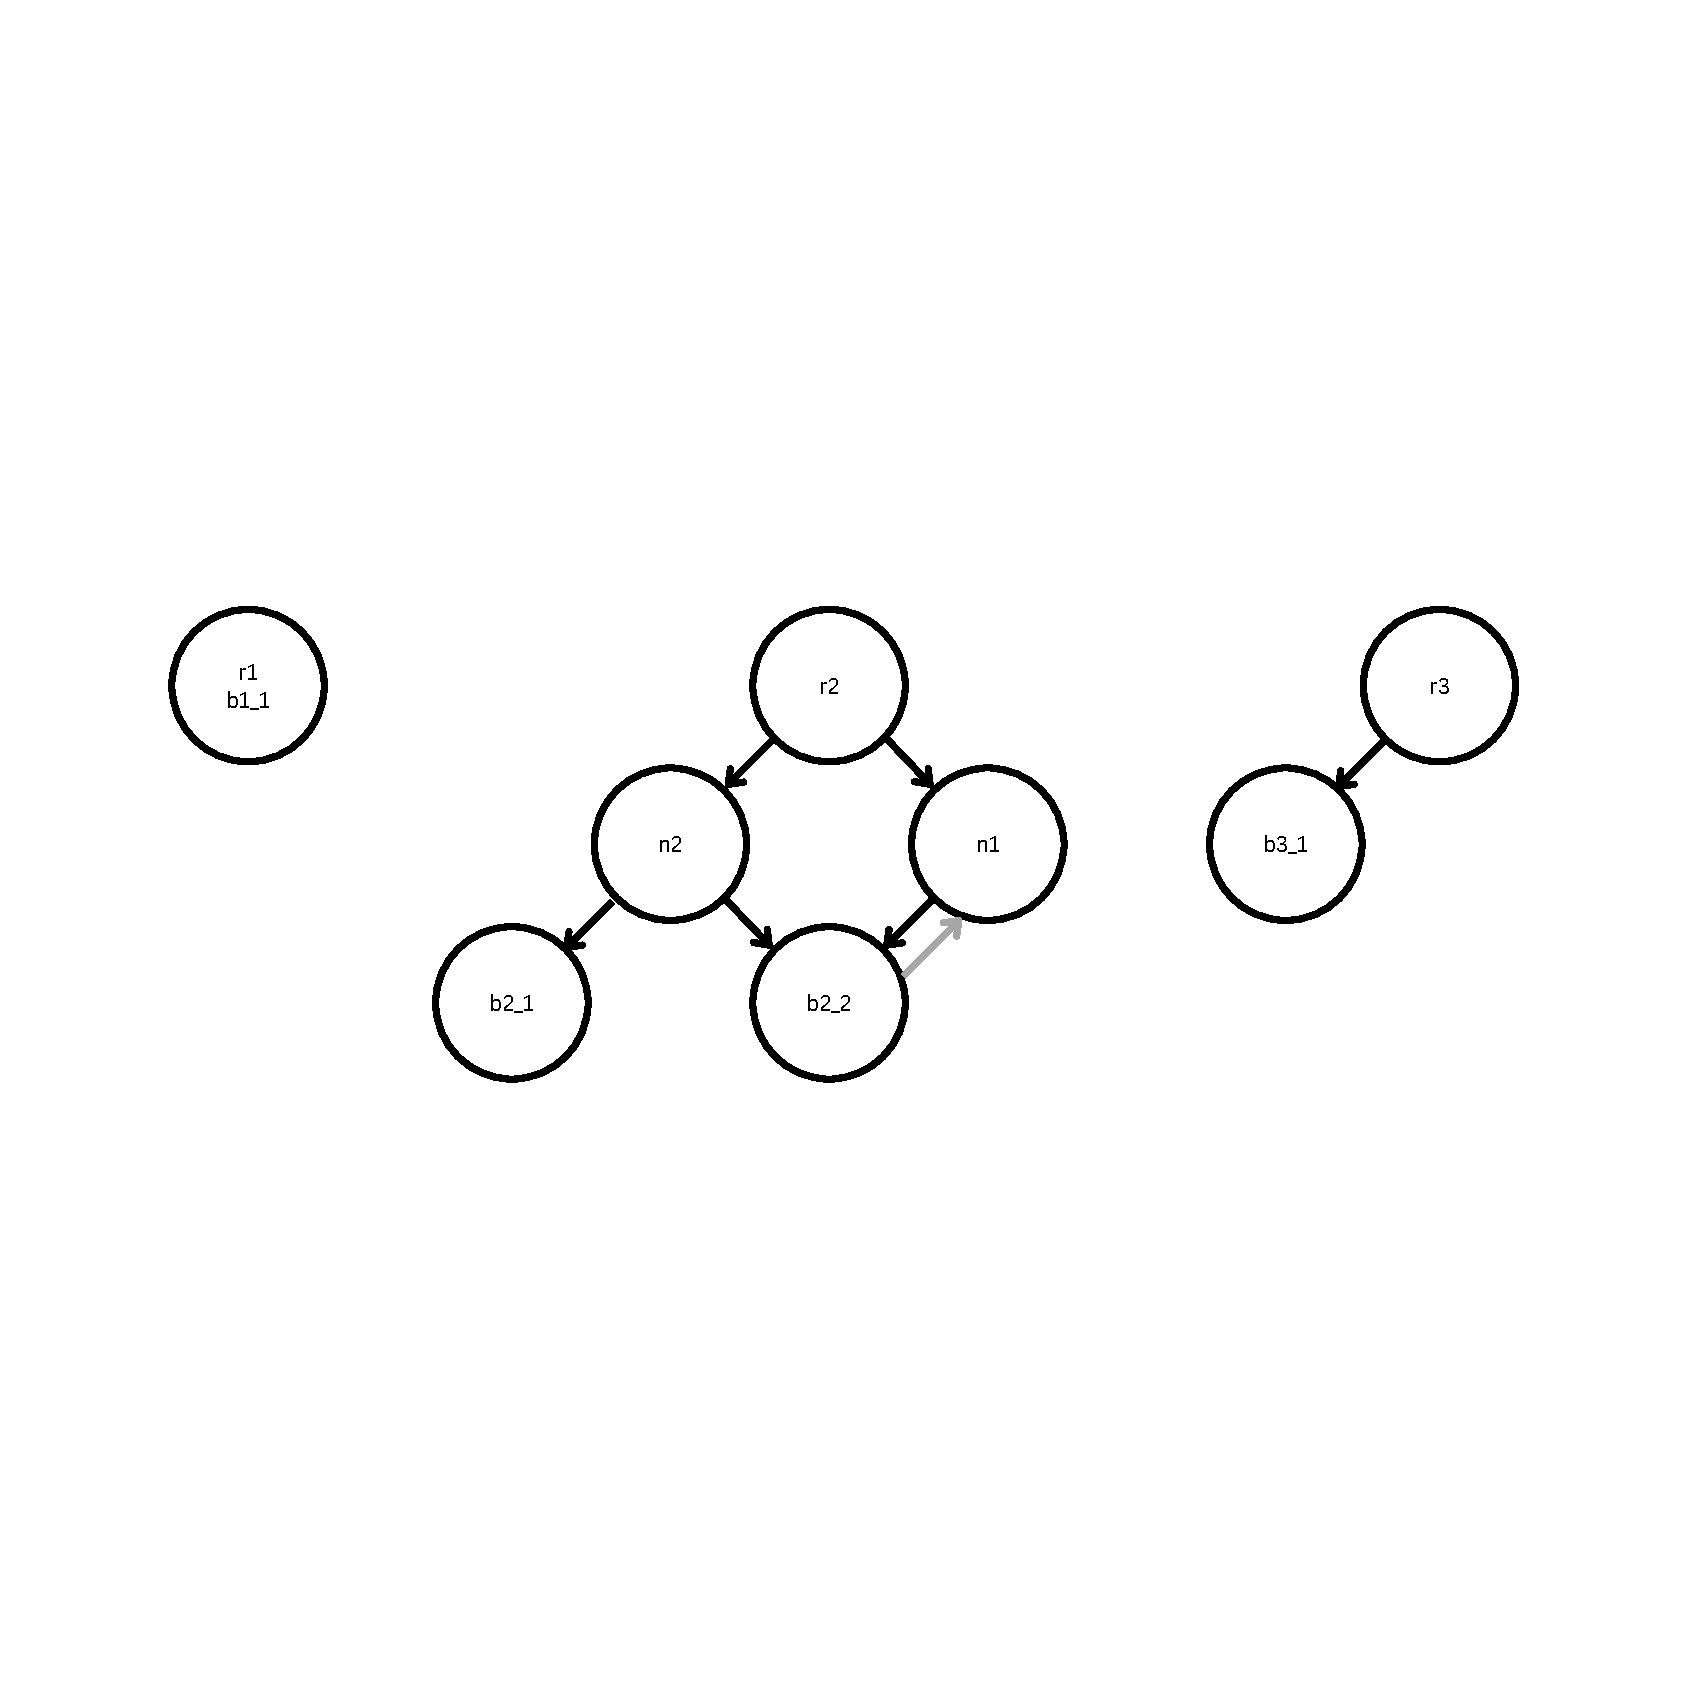
\includegraphics[page=1, trim=0cm 10.25cm 0cm 10.25cm, clip, width=1.00\textwidth]	{assets/coherent_graph.pdf}
	\end{figure}

	Zij $r_i$ ($i \in \mathbb{N}$) wortel van subgraaf $i$ en ${b_i}_j$ ($i \in \mathbb{N}$)
	blad $j$ van de subgraaf $i$. Merk op dat de blad ${b_2}_2$ bidirectioneel verbonden is
	met node $n_1$ en nog steeds als blad wordt beschouwd.

	Verbind vervolgens alle bladeren van elke subgraaf $i$ met hun wortel:
	\begin{figure}[htbp]
		\centering
		\includegraphics[page=2, trim=0cm 10.25cm 0cm 10.25cm, clip, width=1.00\textwidth]	{assets/coherent_graph.pdf}
	\end{figure}

	Blad ${b_1}_1$ wordt niet met de wortel verbonden omdat die op zich zelf een wortel is.
	Daarna doorloop je de wortels $r_i$ en maak je bidirectionele bogen (telkens 2 bogen)
	tussen elk paar wortels:

	\begin{figure}[htbp]
		\centering
		\includegraphics[page=3, trim=0cm 10.25cm 0cm 10.25cm, clip, width=1.00\textwidth]	{assets/coherent_graph.pdf}
	\end{figure}

	De resultaat is een samenhangende graaf waarin je uit elke top elke andere top
	kan bereiken.
\pagebreak

	\chapter{SkewHeap}
	De meest cruciale bewerking in elke heap is naar mijn mening de $merge$-bewerking. Mijn
	implementatie van de skew heap maakt gebruik van het algoritme beschreven in het
	\textbf{boek 4.3.1} (p.77). De skew heap zelf is geïmplementeerd met referenties naar
	twee kinderen (links en rechts), die op zichzelf van het type skew heap zijn. De gehele
	heap bestaat dus feitelijk uit een node met referenties naar de kinder-skew heaps
	(recursieve definitie).

	\begin{lstlisting}[language=Java]
	public class SkewHeap<P extends Comparable<P>, V> implements PriorityQueue<P, V> {
		private SkewHeap<P, V> left;
		private SkewHeap<P, V> right;
		...
	}
\end{lstlisting}

	De \textsf{decreaseKey} wordt normaal opgeroepen op een object die volgende type implementeert:
	\mbox{$QueueItem<P\ extends\ Comparable<P>,\ V>$}.\newline
	Daarom heb ik een implementatie $HeapItem$ gemaakt die
	als veld $item$ wordt opgeslagen in de skew heap.
	HeapItem moet weten welke node (skew deel-heap) op de hoogte gebracht moet worden dat de
	key decreased is om de skew heap eigenschappen in heel de heap te behouden. Eerst had de
	HeapItem een referentie naar de SkewHeap object (node waarin die item zit) en riep die
	verder \textsf{decreaseKey} op op een skew heap object.
	Er was een probleem: de \textsf{decreaseKey}-functie binnen de SkewHeap-klasse moest public zijn, wat resulteerde in een minder goede encapsulatie van de SkewHeap-klasse. Later vond ik echter een betere oplossing om de heap te laten 'fixen' na een \textsf{decreaseKey} van een item: elk item heeft nu een verwijzing naar een \textit{fixheap}-functie uit de SkewHeap-klasse.

	\begin{lstlisting}[language=Java]
	private Runnable decreaseKeyFunction;
\end{lstlisting}

	Als deze functie $null$ is, betekent dit dat het item uit de heap is verwijderd. Nu kan de \textsf{decreaseKey} slechts op één specifieke plaats worden opgeroepen: op het object van HeapItem.

	De grootte van de heap kan op drie verschillende manieren worden bepaald:
	- Door caching tijdens toevoegen/verwijderen\newline
	- Recursief: 1 + (size linker-heap) + (size rechter-heap)\newline
	- Recursief-iteratief: gebruik van $Stack<T>$ om recursie te vermijden\newline


	Laatste implementatie was een omweg om de $StackOverflowExceptions$ te vermijden voor te diepe (ongebalanceerde) skew heaps.

	Om te testen of alle heap-eigenschappen altijd voldaan zijn heb een functie gemaakt die
	recursief nagaat of elke node beide/geen kinderen heeft, oftewel alleen linker kind.

	\section{Benchmarks}

	\subsection{Add item}

	Het invoegen van een item in een skew heap is een bewerking die over het algemeen weinig kost, zoals te zien is in de benchmarkresultaten hieronder:

\begin{figure}[htbp]
	\centering
	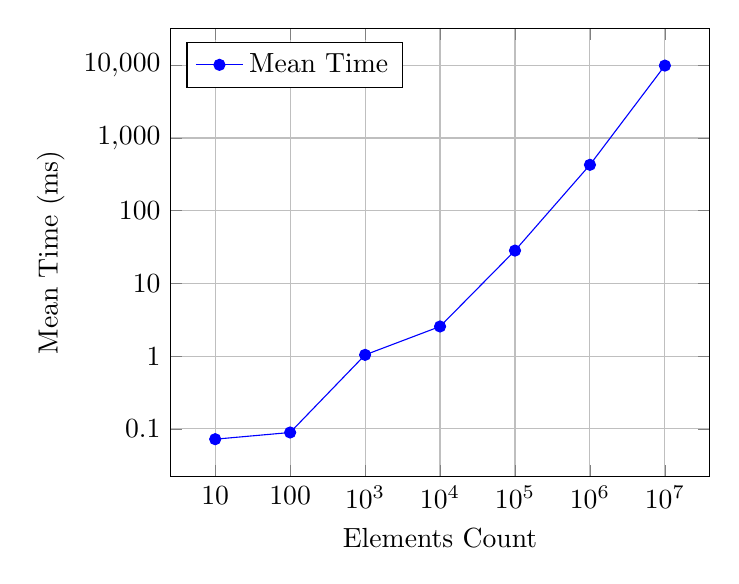
\begin{tikzpicture}
		\begin{axis}[
			xlabel={Elements Count},
			ylabel={Mean Time (ms)},
			legend pos=north west,
			grid=both,
			xmode=log,
			ymode=log,
			log ticks with fixed point,
			xtick={10, 100, 1000, 10000, 100000, 1000000, 10000000},
			xticklabels={$10$, $100$, $10^3$, $10^4$, $10^5$, $10^6$, $10^7$},
			ymajorgrids=true,
			yminorgrids=false,
			yminorticks=false,
			xmajorgrids=true,
			xminorgrids=false,
			xminorticks=false,
			]

			% Data points
			\addplot[blue, mark=*] coordinates {
				(10, 0.072) (100, 0.089) (1000, 1.04) (10000, 2.556) (100000, 28.287) (1000000, 427.835) (10000000, 9918.219)
			};

			% Add legend
			\legend{Mean Time}

		\end{axis}
	\end{tikzpicture}
	\caption{SkewHeap elementen toevoegen}
\end{figure}

	Wanneer de invoergrootte wordt verhoogd met een factor van 10, neemt de uitvoeringstijd
	als volgt toe: (Zie tabel 2.1)

\begin{table}[htbp]
	\centering

	\label{tab:uitvoeringstijd}
	\begin{tabular}{cc}
		\toprule
		\textbf{Vergroting van invoergrootte} & \textbf{Toename van uitvoeringstijd} \\
		\midrule
		1x naar 1000x & ... \\
		1.000x naar 10.000x & x2.5 \\
		10.000x naar 100.000x & x11.1 \\
		100.000x naar 1.000.000x & x15.1 \\
		1.000.000x naar 10.000.000x & x23.2 \\
		... & ... \\
		\bottomrule
	\end{tabular}
	\caption{Toename van uitvoeringstijd bij vergroting van de invoergrootte}
\end{table}

	Die toename ziet er logaritmisch (per bewerking) uit, wat in $O(n\log n)$ resulteert op
	$n$ reeks toevoegingen. Dat is ook te zien op een exponentieel grafiek die voor grote $n$
	linear is.

	\subsection{Decrease key en poll}

	Tijdens testen merkte ik dat decrease key ook op de root van de heap opgeroepen kan
	worden, standaart algoritme zou dan de kinderen van de root mergen en dan de resulterende heap de linker kind van root maken. Zie volgende schets met keys: $z \ge x \ge y \ge a$.

	\begin{figure}[H]
		\centering
		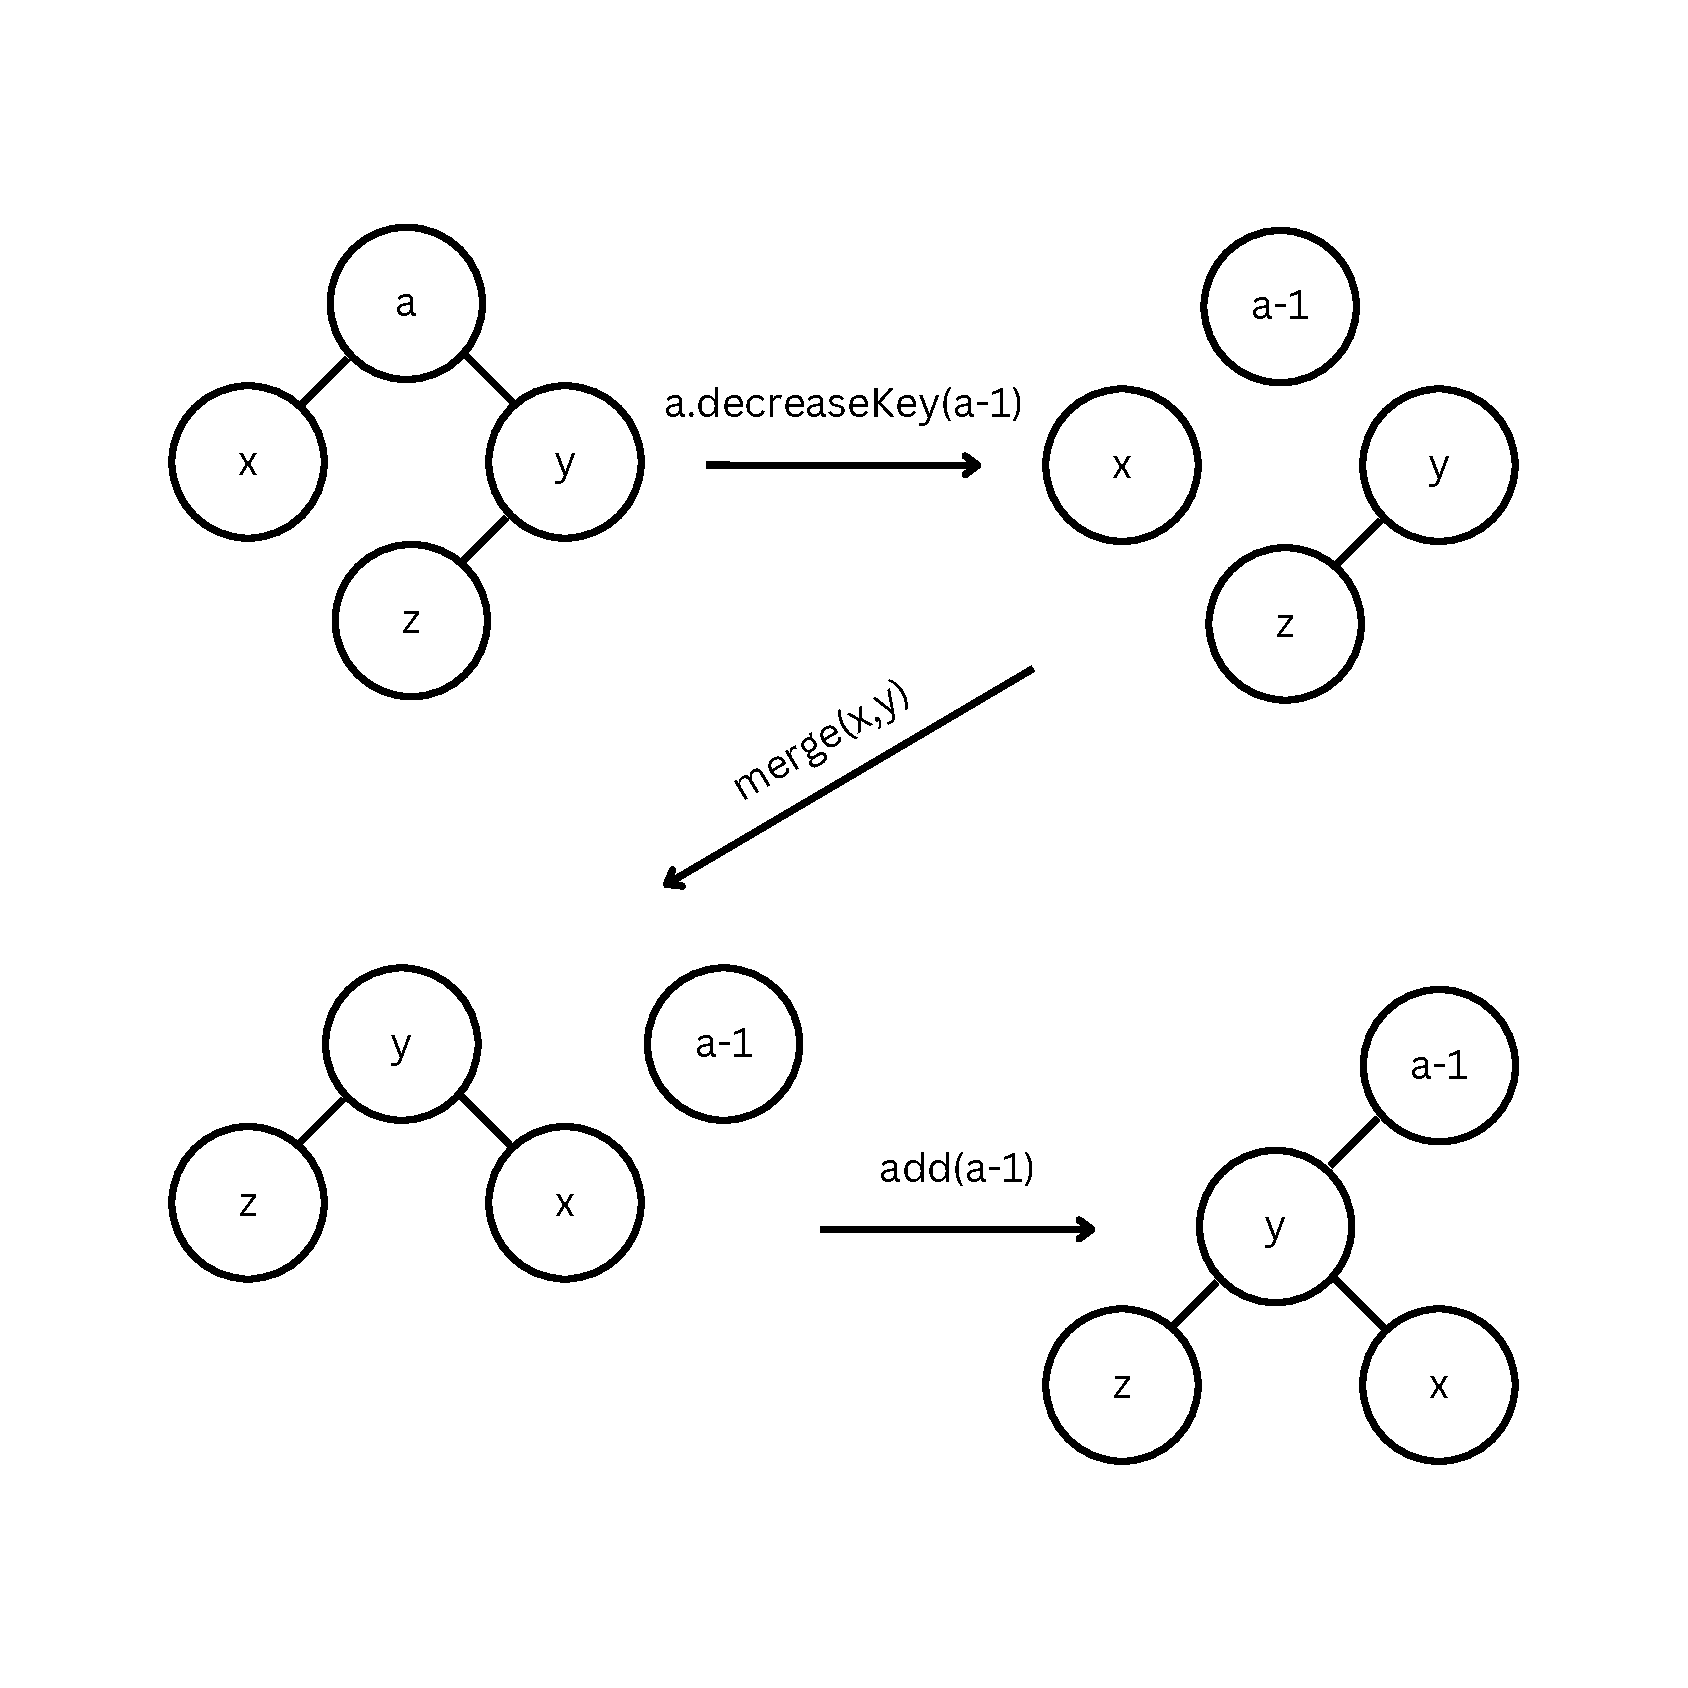
\includegraphics[height=0.45\textheight]{assets/skew_decrease_key_poll.pdf}
	\end{figure}
\pagebreak

	Ik vond dat onnodig, vooral als de deelboom van $x$ meerdere elementen zou bevatten.
	Daarom heb ik een statische variabele toegevoegd waarmee de gebruiker kan kiezen of er al
	dan niet moet worden samengevoegd voor de \textsf{decreaseKey} bewerking op de root.

	\begin{lstlisting}[language=Java]
	public static boolean reMergeRoot = false;
\end{lstlisting}

	Dan wou ik deze verbetering benchen door eerst 2 willekeurige elementen te decreasen en
	vervolgens een \textsf{decreaseKey} op de root uit te voeren, gevolgd door \textsf{poll}.
	Volgende grafieken tonen mijn benchmarks: deze methode is sneller, maar alleen voor
	kleine heaps (tot 100.000 elementen).

\begin{figure}[htbp]
	\centering
	\begin{minipage}{\textwidth}
		\centering
		\begin{subfigure}{0.45\textwidth}
			\centering
			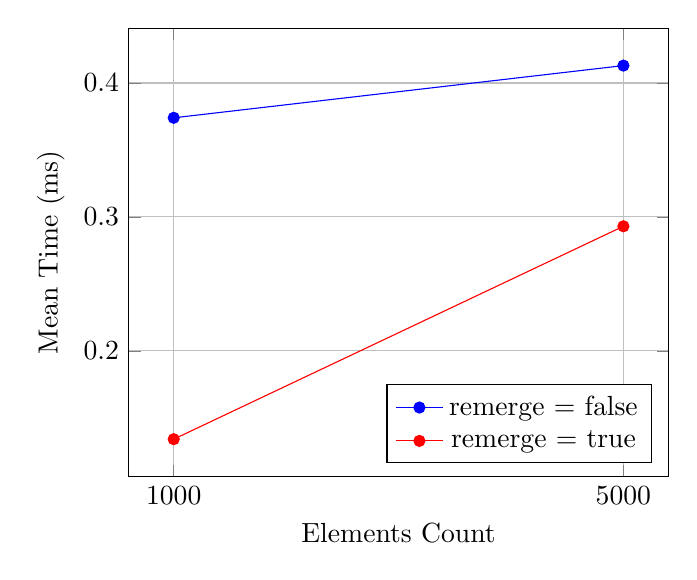
\begin{tikzpicture}
				% First plot
				\begin{axis}[
					xlabel={Elements Count},
					ylabel={Mean Time (ms)},
					legend pos=south east,
					grid=both,
					xmode=log,
					log ticks with fixed point,
					xtick={1000, 5000},
					xticklabels={1000, 5000},
					]

					% remerge = false data points
					\addplot[blue, mark=*] coordinates {
						(1000, 0.374)
						(5000, 0.413)
					};

					% remerge = true data points
					\addplot[red, mark=*] coordinates {
						(1000, 0.134)
						(5000, 0.293)
					};

					% Add legend
					\legend{remerge = false, remerge = true}

				\end{axis}
			\end{tikzpicture}
		\end{subfigure}
		\hfill
		\begin{subfigure}{0.45\textwidth}
			\centering
			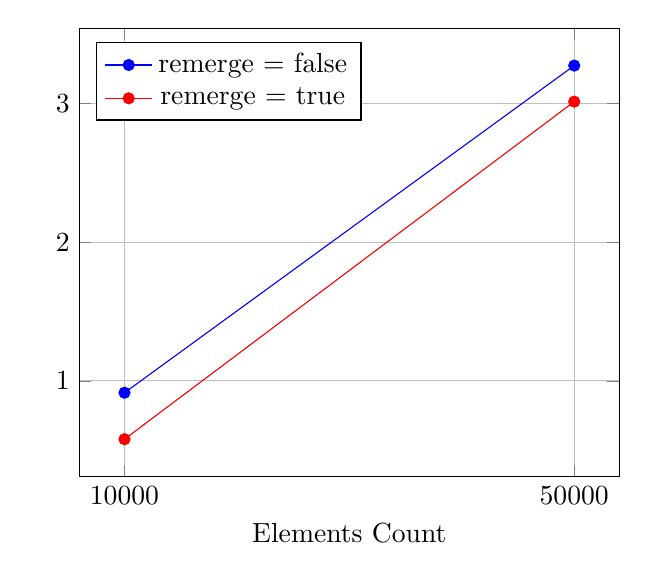
\begin{tikzpicture}
				% Second plot
				\begin{axis}[
					xlabel={Elements Count},
					ylabel={\ },
					legend pos=north west,
					grid=both,
					xmode=log,
					log ticks with fixed point,
					xtick={10000, 50000},
					xticklabels={10000, 50000},
					]

					% remerge = false data points
					\addplot[blue, mark=*] coordinates {
						(10000, 0.915)
						(50000, 3.274)
					};

					% remerge = true data points
					\addplot[red, mark=*] coordinates {
						(10000, 0.58)
						(50000, 3.014)
					};

					% Add legend
					\legend{remerge = false, remerge = true}

				\end{axis}
			\end{tikzpicture}
		\end{subfigure}
	\end{minipage}

	\bigskip

	\begin{minipage}{\textwidth}
		\centering
		\begin{subfigure}{0.45\textwidth}
			\centering
			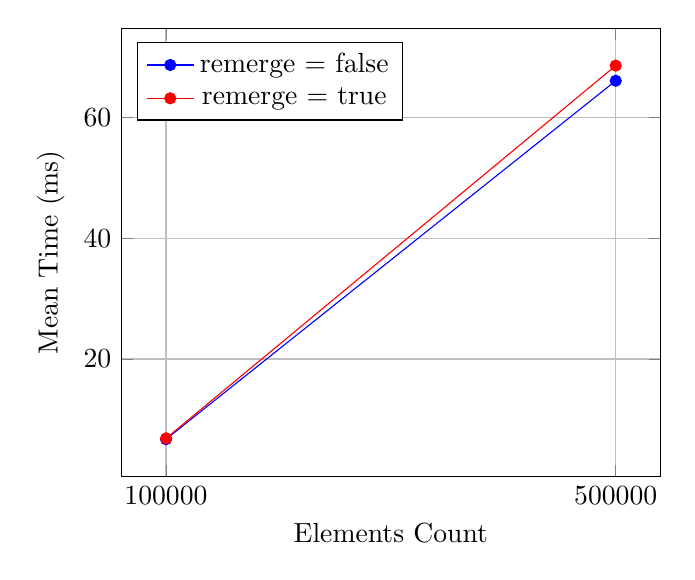
\begin{tikzpicture}
				% Third plot
				\begin{axis}[
					xlabel={Elements Count},
					ylabel={Mean Time (ms)},
					legend pos=north west,
					grid=both,
					xmode=log,
					log ticks with fixed point,
					xtick={100000, 500000},
					xticklabels={100000, 500000},
					]

					% remerge = false data points
					\addplot[blue, mark=*] coordinates {
						(100000, 6.732)
						(500000, 66.028)
					};

					% remerge = true data points
					\addplot[red, mark=*] coordinates {
						(100000, 6.874)
						(500000, 68.538)
					};

					% Add legend
					\legend{remerge = false, remerge = true}

				\end{axis}
			\end{tikzpicture}
		\end{subfigure}
	\end{minipage}
	\caption{\textbf{2x} \textit{random decreaseKey} + \textbf{1x} \textit{decreaseKey op
			root met poll}}
\end{figure}

	\pagebreak

	\section{Complexiteit van Decrease key}
	Voor beide bewijzen zullen wij Stelling 16 uit het boek AD2 2023 gebruiken en
	ook de definities die daar werden geïntroduseerd.

	\subsubsection{Algoritme 1}
	\begin{quote}
		Decrease key op skew heap $S$:

		De deelboom $S_{v}$ met als wortel $v$ wordt verwijderd uit de heap. Dan wordt het pad van
		$v$ naar de wortel overlopen. Als een top op dat pad $v$ in zijn linkerdeelboom heeft en
		een rechterkind heeft, dan worden zijn kinderen gewisseld. Zo blijft het resultaat een
		skew heap. De wortel $v$ wordt \underline{kleiner}, en
		$S_{v}$ wordt terug gemerged met de originele heap.
	\end{quote}

	\textbf{Propositie:}

	De geamortiseerde complexiteit van een reeks van $n$ bewerkingen
	(toevoegen, wortel verwijderen, decrease key) op een initieel lege skew heap is $O(n\ \log n)$.
	\newline

	\textbf{Bewijs/Tegenvoorbeeld:}

	Deze algoritme voor decrease key maakt gebruik van mergebewerking
	maar ook een bewerking die op het pad naar de wortel kinderen
	verwisseld die wij vanaf nu $fixpath$-bewerking zullen noemen.
	\newline

	Uit Stelling 16 weten wij dat complexiteit van een mergebewerking geamortiseerd
	$O(\log n)$ per bewerking is maar wat is de complexiteit van $fixpath$
	eigenlijk?
	\newline

	Na een aantal pogingen vinden wij een reeks bewerkingen die ervoor zorgen dat er veel slechte toppen gemaakt worden tijdens onze $fixpath$.

	Aan een lege skew heap $S$ voegen wij eerst $n$ elementen in een
	gegeven volgorde toe (z.v.v.a. n is even):
	$n-1$ dan $n$, dan $n-3$ en dan $n-2$ ... dan $1$ en dan $2$.
	\newline

	Algemeen: $add\_semi\_descending(i) = n - i + (-1)^i + 1$

	Voeg $n$ elementen toe: $\forall\ i\in \{1..n\}\ .\ add\_semi\_descending(i)$
	\newline

	Resultaat van deze toevoegingen zie je op het figuur \underline{rechts} onderaan.
	Die toevoegingen worden in een constante tijd uitgevoerd omdat wij telkens
	\underline{hoogstens één} vergelijking op de rechter pad uitvoeren
	(eventueel gevolgd door 1 swap van kinderen van de wortel),
	dus $O(n)$ voor reeks van $n$ bewerkingen.
	\newline

	\textbf{Stap 1}: Wij voegen een key $N > n$ toe ($S_v = S_N$) zodat onze $S$ de \underline{linkse} heap wordt (op figuur onderaan).

	\textbf{Stap 2}: Wij passen de bewerking decrease key op onze key $v = N$ toe dat
	eerst de $S_N$ uit de heap verwijdert en dan $fixpath$ bewerking op de linkse pad van $S$ uitvoert
	wat in \underline{rechtse} heap resulteert. Daarna mergen wij $S_N$ terug met $S$ wat terug in
	\underline{linkse} heap resulteert.

	Wij passen nu stap 2 $n$ keer toe en zien hier dat
	wij telkens met elke decrease key $O(n)$ swaps nodig hebben:
	\newline
	$\mathbf{1}$ (verwijderen van $S_N$) $+$ $\mathbf{\frac{n}{2}}$(links -> rechts) $+$
	\newline
	$\mathbf{1}$ (toevoegen van $S_N$) $+$ $\mathbf{\frac{n}{2}}$(rechts -> links)
	\newline
	wat voor reeks van $k$ decrease keys bewerkingen in $O(kn)$ resulteert.
	\newline

	Stel een aantal bewerkingen $m$ met eerst $n$ toevoegingen zoals in definieërd boven
	en dan $k > n$ decrease keys dan is $m = n + k$ en de complexiteit is: $O(n) + O(kn)$.
	Aangezien wij alleen kijken voor $k > n$ kunnen wij eerste term laten
	vallen en 2de term herschrijven als: $\Omega(n^2)$

	Dat betekent dat geamortiseerde complexiteit (met algoritme 1 voor decrease key) van een reeks van $n$ bewerkingen
	(toevoegen, wortel verwijderen, decrease key) op een initieel lege skew heap \textbf{niet} $O(n\ \log n)$ kan zijn.

	\begin{flushright}
		$\Box$
	\end{flushright}

	\begin{figure}
	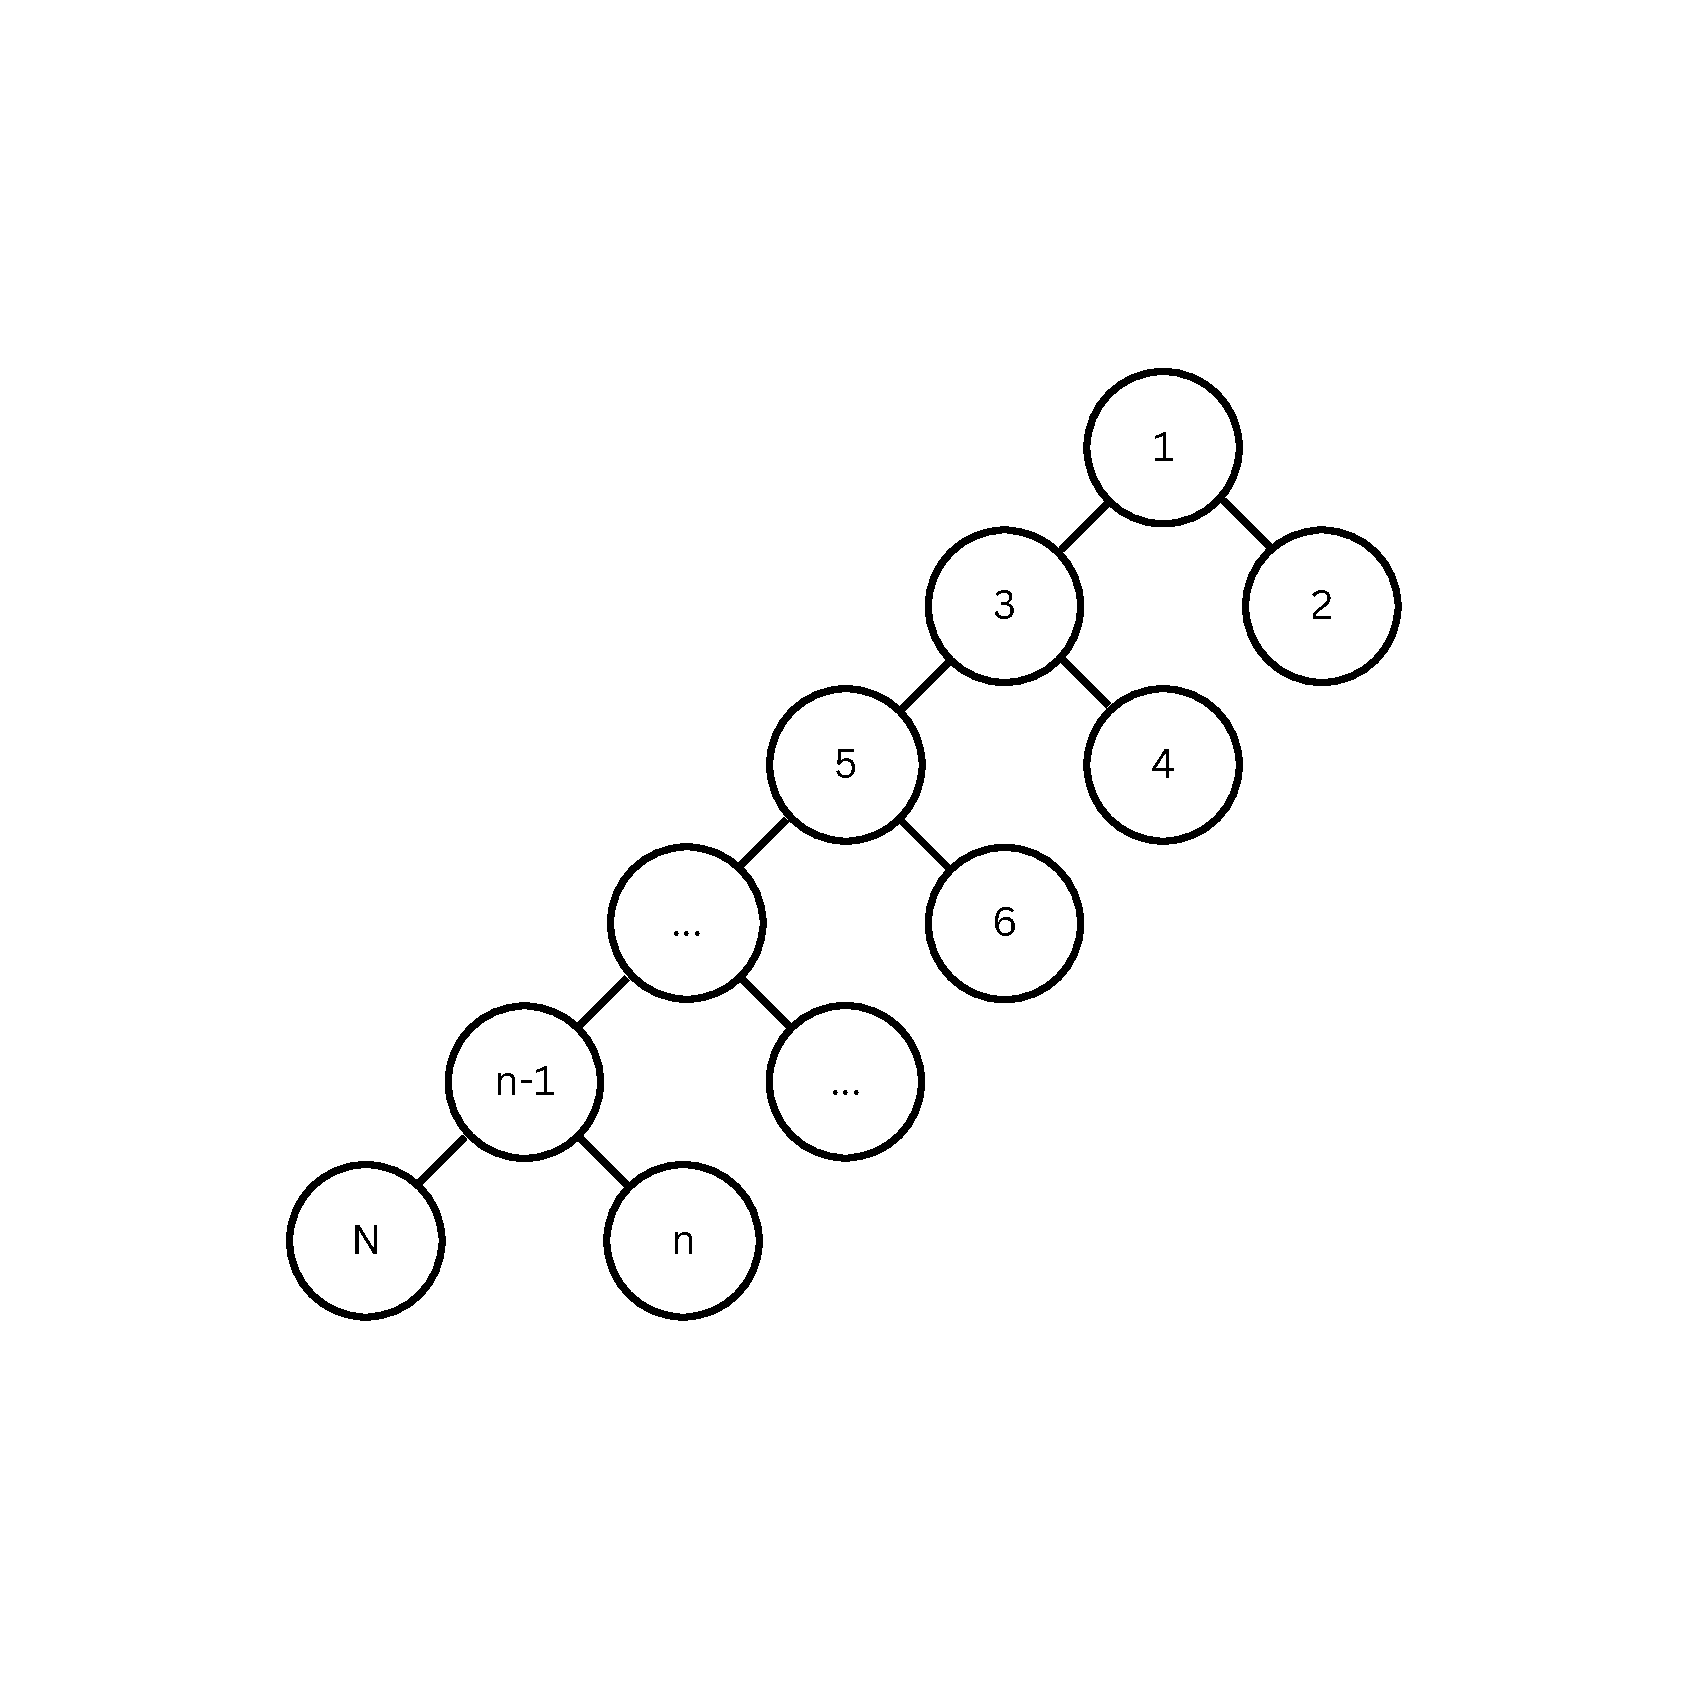
\includegraphics[height=0.3\textheight] {assets/skew_heap_init.pdf}
	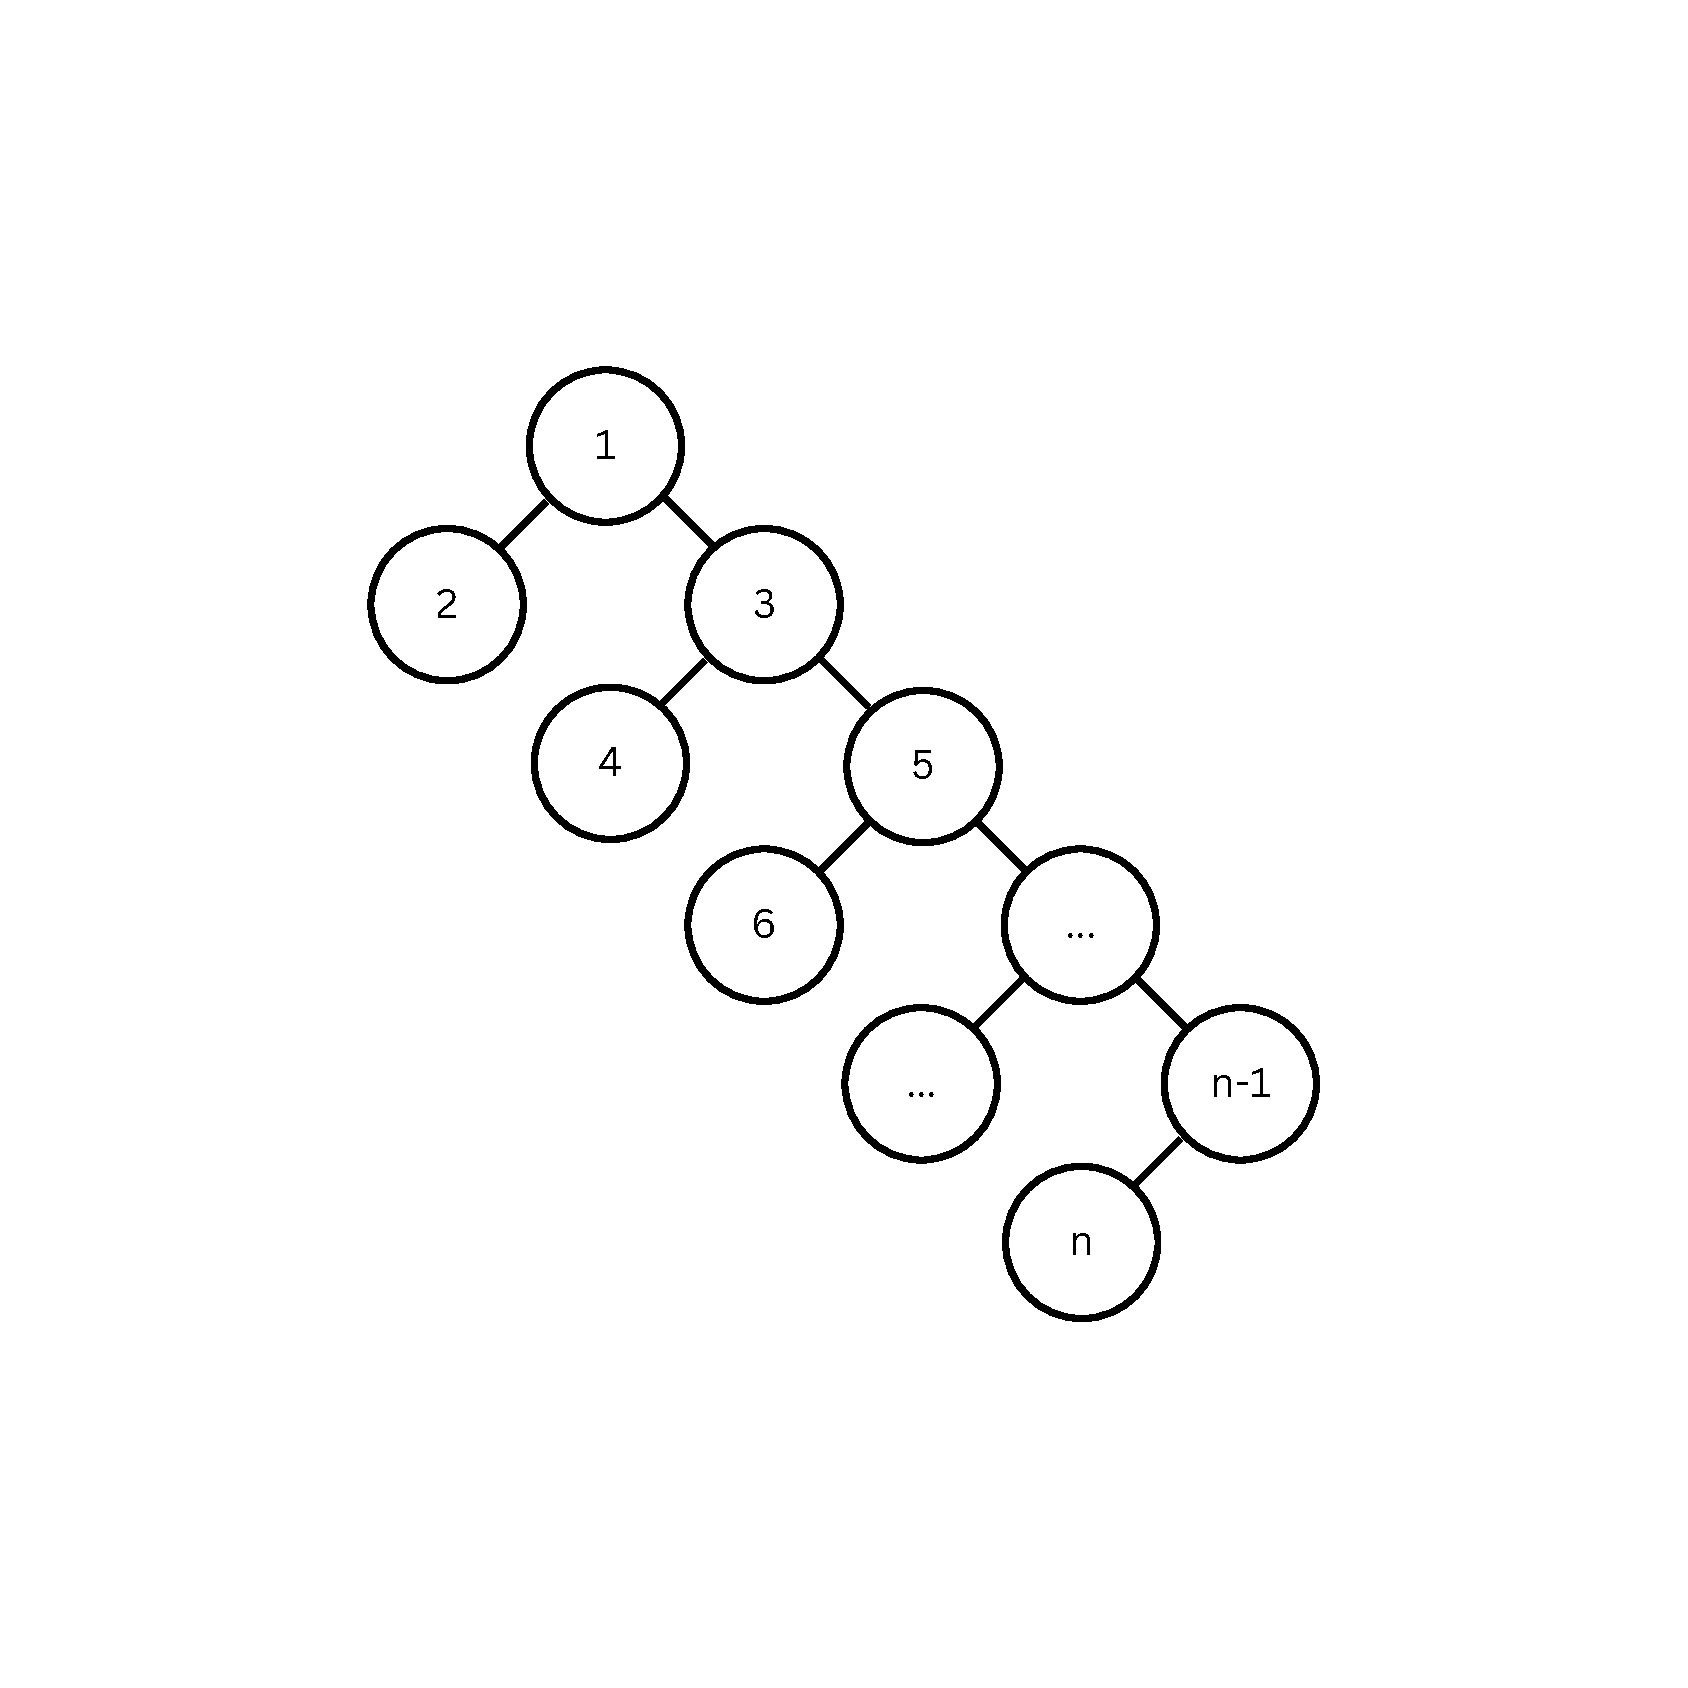
\includegraphics[height=0.3\textheight] {assets/skew_heap_after_remove.pdf}
	\caption{Skew heap voor en na het verwijderen van N}
	\end{figure}

	\subsubsection{Algoritme 2}
	\begin{quote}
		Decrease key op skew heap $S$:

		De deelboom $S_{v}$ met als wortel $v$ wordt verwijderd uit de heap. Dan wordt de wortel
		(dit is top $v$) verwijderd uit $S_{v}$ met de operatie uit de cursus. Het resultaat wordt
		terug in $S$ geplaatst, met de nieuwe wortel op de plaats waar $v$ zat. Er wordt bij het
		terugplaatsen niet gemerged en er worden geen kinderen gewisseld. Uiteindelijk wordt de
		top $v$ met de heap $S$ gemerged.
	\end{quote}

	\textbf{Propositie:}

	De geamortiseerde complexiteit van een reeks van $n$ bewerkingen
	(toevoegen, wortel verwijderen, decrease key) op een initieel lege skew heap is $O(n\ \log n)$.
	\newline

	\textbf{Bewijs/Tegenvoorbeeld:}

	Zoals in de Stelling 16 vermeld staat:
	\begin{quote}
		Het maakt het niet uit of wij de toevoegen en wortel verwijderen met een
		mergebewerking zouden samenvatten, de kost zou gewoon die van
		de mergebewerking zijn. (1)
	\end{quote}

	Wij baseren ons op de deelresultaten van Stelling 16 en voegen een
	extra deelresultaat toe.
	\newline

	\textbf{Deelresultaat 5:}
	Als op een top $S_v$ in een skew heap $S$ in de verzameling $D$ een decrease
	key bewerking wordt	toegepast en het resultaat $D'$ is dan geldt:
	$\Phi (D') - \Phi (D) = k$
	met $k$ aantal goede toppen die in $D'$ slecht worden.
	\newline

	De echte kost van decrease key zal $O(1)$ zijn wegens punt 1 (bovenaan) die zegt
	dat wij geen rekening moeten houden met mergen. Hier zal namelijk 2 keer gemerged moeten worden.

	\begin{table}[H]
		\begin{tabular}{l|l|l}
			\multicolumn{1}{c}{}                                                                     & echte kost & gewijzigde kost \\ \hline
			\begin{tabular}[c]{@{}l@{}}één nieuwe skew\\ heap met 1 element\\ toevoegen\end{tabular} & 1          & \begin{tabular}[c]{@{}l@{}} $1 + \Phi(D') - \Phi(D) = 1$ \end{tabular} \\ \hline
			\begin{tabular}[c]{@{}l@{}}de wortel van één\\ skew heap verwijderen\end{tabular}        & 1          & \begin{tabular}[c]{@{}l@{}}$1 + \Phi(D' ) - \Phi(D) \leq 1$\end{tabular} \\ \hline
			\begin{tabular}[c]{@{}l@{}}twee skew heaps in\\ de verzameling mergen\end{tabular}       & g+s        & \begin{tabular}[c]{@{}l@{}}$g + s + \Phi(D' ) - \Phi(D) \leq g + s + (g - s) = 2g$ \\ $= O(\log m)$ met $m$ aantal bewerkingen \end{tabular} \\ \hline
			\begin{tabular}[c]{@{}l@{}}decrease key uitvoeren\\ op één top in S\end{tabular}         & 1          & $1 + \Phi(D') - \Phi(D) = 1 + k$ (Deelresultaat 5)
		\end{tabular}
	\end{table}

	Hoe groot is nu k? Wij maken gebruik van \textbf{Lemma 1} die zegt dat
	$k \leq \log|S|$ en wij weten dat $|S| \leq m$ met $m$
	aantal bewerkingen.
	\newline

	Dus is $k = O(\log m)$ een bovengrens voor de gewijzigde kost van
	decrease key. Dat impliceert dat $O(m \log m)$ een bovengrens
	voor de geamortiseerde complexiteit van een arbitraire rij van
	$m$ bewerkingen op een initieel lege verzameling van skew heaps is.
	\newline

	\textbf{Lemma 1:} Als $k$ het aantal goede toppen die na het verwijderen van top $v$ uit de heap $S$ slecht worden dan is
	$k \leq \log |S|$.
	\newline

	\textbf{Bewijs:}

	Om in te zien hoeveel goede toppen na het verwijderen van top $v$ slecht worden kijken
	wij wanneer één top slecht wordt.
	Stel $S_o$ is de hoogste top die goed was en slecht is geworden ($|S_o| \leq |S|$).
	Dat gebeurt namelijk als een top $S_o$ even veel kinderen links: $|S_l| = l$ en rechts:
	$|S_r| = r$ had ($r=l$), dus na het verwijderen van $v$ aantal kinderen $l = r - 1$.
	\newline
	Wij bewijzen dat $k \leq \log |S|$ met inductie.
	\newline

	\textbf{Inductiebasis:} Bewijs voor $k = 1$:

	Met $k = 1$ bestaat er exact één top $S_o$ in $S$ met $|S_r| = |S_l|$
	(ook $|S_o| \leq |S|$).
	Na het verwijderen van $v$ is $|S'_l| < |S_r|$ of
	meer specifiek: $|S'_l| = |S_r| - 1$.
	\newline
	Wij weten dat $S_r$ minstens 1 top heeft die in $S_l$ met $v$ correspondeerde (voor de voorwaarde $|S_r| = |S_l|$). Dus $|S_r| \geq 1$.
	\newline
	Deelboom van $S_r$ samen met top $S_o$ geven: $|S_o| \geq 2$ (ook: $ 1 \leq \log |S_o|$).
	\newline
	Zo geldt: $1 \leq \log |S_o| \leq \log |S|$.
	\newline

	\textbf{Inductiehypothese:} $n \leq \log |S|$.
	\newline

	\textbf{Inductiestap:} Bewijs voor $k = n + 1$:

	Wij weten dat $r = l$ dus vervangen wij $|S_o| = |S_l| + |S_r| = 2|S_l|$:
	\newline
	Zo geldt: $n + 1 \leq \log 2|S_l|$.
	\newline
	Dan: $n + 1 \leq \log |S_l| + 1$
	\newline
	Dan: $n \leq \log |S_l|$ wat onze inductie hypothese is omdat $S_o$ de \textbf{hoogste} top was en omdat wij dat reduceren tot $n$.

	\begin{flushright}
	$\Box$
	\end{flushright}

	\chapter{My Heap}

	Voor mijn implementatie van de MyHeap heb ik de keuze gemaakt om de Pairing Heap te gebruiken, aangezien deze eerst de snelste leek te zijn tussen de heaps die relatief eenvoudig te implementeren zijn. Net zoals in het geval van de SkewHeap, veroorzaken sommige recursieve bewerkingen een $StackOverflowException$. Om dit te omzeilen, heb ik een aantal iteratieve alternatieven ontwikkeld. Een van deze iteratieve bewerkingen is de $twoPassMerge$, die een cruciale rol speelt in de definitie van PairingHeap. Bovendien is er in de 'oplossing'-map ook $MyPriorityQueueOld$ aanwezig, mijn eerste poging om een PairingHeap te implementeren.

	$MyPriorityQueueOld$ houdt de lijst van siblings bij in plaats van alleen
	linker- en rechter-siblings. Deze implementatie zorgt voor een snelle oplossing voor veel randgevallen, waardoor het gemakkelijk te implementeren was, maar het was niet correct. Tijdens \textsf{decreaseKey} wordt de volgende regel uitgevoerd:
	\begin{lstlisting}[language=Java]
		siblings.remove(this);
\end{lstlisting}

	Met behulp van een profiler heb ik waargenomen dat deze regel vaak een zeer dure bewerking is. Dit is gemakkelijk te begrijpen omdat de lijst erg groot kan worden, en remove $O(n)$ is met $n$ elementen in de lijst.

	Later heb ik de PairingHeap herschreven om alleen referenties naar hun linker- en rechter-siblings op te slaan. Deze referenties moeten vaak worden bijgewerkt en over het algemeen is er meer 'boekhouding' dan in de 'Old' versie.


	\section{Benchmarks}

	Benchmarks voor $add$ bewerking hebben weinig zin omdat die vast $O(1)$ zijn dus wij
	zullen direct \textsf{decreaseKey} met \textsf{poll} benchmarken.
\pagebreak
	\subsection{Decrease key en poll}


\begin{figure}[htbp]
	\centering
	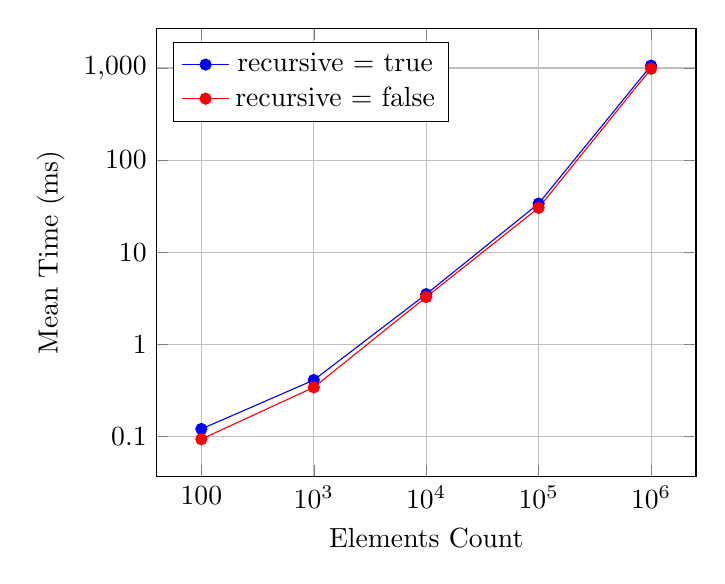
\begin{tikzpicture}
		\begin{axis}[
			xlabel={Elements Count},
			ylabel={Mean Time (ms)},
			legend pos=north west,
			grid=both,
			xmode=log,
			ymode=log,
			log ticks with fixed point,
			xtick={100, 1000, 10000, 100000, 1000000},
			xticklabels={$100$, $10^3$, $10^4$, $10^5$, $10^6$},
			ymajorgrids=true,
			yminorgrids=false,
			yminorticks=false,
			xmajorgrids=true,
			xminorgrids=false,
			xminorticks=false,
			]

			% Data points
			\addplot[blue, mark=*] coordinates {
				(100, 0.12)
				(1000, 0.408)
				(10000, 3.496)
				(100000, 33.681)
				(1000000, 1062.349)
			};

			% Data points
			\addplot[red, mark=*] coordinates {
				(100, 0.093)
				(1000, 0.34)
				(10000, 3.253)
				(100000, 30.271)
				(1000000, 981.315)
			};

			% Add legend
			\legend{recursive = true, recursive = false}

		\end{axis}
	\end{tikzpicture}
	\caption{Decrease Key en poll}
\end{figure}

	Bovenaan zien we dat de iteratieve methode niet alleen veilig is tegen
	$StackOverflowException$, maar ook dat deze klein beetje sneller is dan de eenvoudige
	recursieve \textsf{twoPassMerge}.

	Opmerkelijk is dat de functie lijkt te groeien als een exponentiële functie op de
	exponentiële y-as. Dit suggereert dat de verwachte complexiteit hoger is dan $O(\log n)$
	per bewerking.

	We kunnen al vaststellen dat na het uitvoeren van $n$ \textsf{decreaseKey}-bewerkingen,
	de \textsf{twoPassMerge} dan over $n$ elementen moet itereren. Met andere woorden, veel
	\textsf{decreaseKey}-bewerkingen vertragen onze \textsf{poll}-bewerking.

	\chapter{Shortest Path}

	Voor de implementatie van mijn shortest path heb ik A* algoritme gebruikt.
	De implementatie is eenvoudig en "straight forward".

	\section{Benchmarks}

	We kijken verder hoe de A* presteert bij verschillende hoeveelheden edges en met
	verschillende heaps:

\begin{figure}[htbp]
	\centering
		\begin{subfigure}{0.38\textwidth}
		\centering
		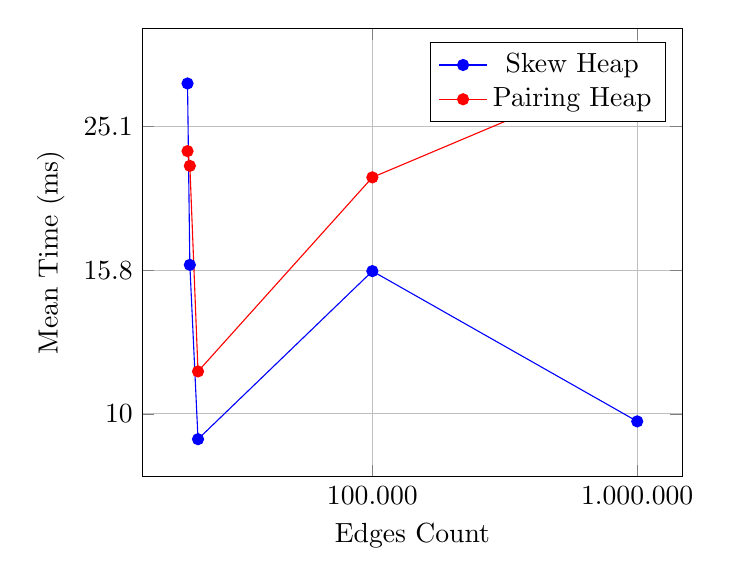
\begin{tikzpicture}
			\begin{axis}[
				xlabel={Edges Count},
				ylabel={Mean Time (ms)},
				legend pos=north east,
				grid=both,
				xmode=log,
				ymode=log,
				log ticks with fixed point,
				xtick={100000, 1000000},
				xticklabels={$100.000$, $1.000.000$},
				ymajorgrids=true,
				yminorgrids=false,
				yminorticks=false,
				xmajorgrids=true,
				xminorgrids=false,
				xminorticks=false,
				]

				% Data points
				\addplot[blue, mark=*] coordinates {
					(20051, 28.833)
					(20459, 16.12)
					(21965, 9.218)
					(100000, 15.799)
					(1000000, 9.759)
				};

				% Data points
				\addplot[red, mark=*] coordinates {
					(20051, 23.21)
					(20459, 22.14)
					(21965, 11.454)
					(100000, 21.338)
					(1000000, 30.537)
				};

				% Add legend
				\legend{Skew Heap, Pairing Heap}

			\end{axis}
		\end{tikzpicture}
		\caption{10.000 nodes}
	\end{subfigure}
	\hfill
	\begin{subfigure}{0.38\textwidth}
	\centering
		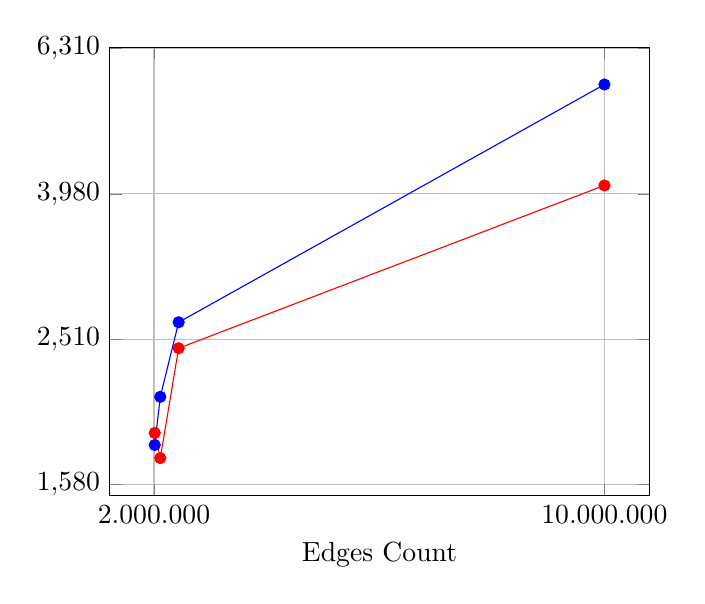
\begin{tikzpicture}
			\begin{axis}[
				xlabel={Edges Count},
				grid=both,
				xmode=log,
				ymode=log,
				log ticks with fixed point,
				xtick={1000000, 2000000, 10000000},
				xticklabels={$10^6$, $2.000.000$, $10.000.000$},
				ymajorgrids=true,
				yminorgrids=false,
				yminorticks=false,
				xmajorgrids=true,
				xminorgrids=false,
				xminorticks=false,
				]

				% Data points
				\addplot[blue, mark=*] coordinates {
					(2004912, 1797.051)
					(2045023, 2093.18)
					(2183966, 2650.666)
					(10000125, 5628.485)
				};

				% Data points
				\addplot[red, mark=*] coordinates {
					(2004912, 1867.183)
					(2045023, 1724.113)
					(2183966, 2441.686)
					(10000125, 4088.545)
				};

			\end{axis}
		\end{tikzpicture}
		\caption{1.000.000 nodes}
	\end{subfigure}
\end{figure}

	Het aantal bogen voor elk van de grafen werd bepaald door het aantal random
	gegenereerde bogen + aantal bogen die werden toegevoegd om de graaf
	samenhangend te maken(met algoritme beschrijven in sectie \textbf{1.2}).
	Dus voor grafiek a:\newline
	100 random + 19.951 verplicht \newline
	1.000 random + 19.459 verplicht \newline
	10.000 random + 11.965 verplicht \newline
	100.000 random + 0 verplicht \newline
	1.000.000 random + 0 verplicht \newline

	We zien bij grafiek a dat A* het snelst is als het aantal bogen "dicht" bij het aantal
	nodes is of wanneer de graaf (bijna) compleet is (wat altijd triviale oplossingen
	oplevert met padlengte = 1).

	Grafiek b ziet er anders uit en ik vermoed dat als het aantal bogen ${10^6}^2$ zal
	zal bereiken dat de uitvoeringstijden op dezelfde manier zullen afnemen omdat de graaf
	bijna compleet zal worden.

	In het algemeen is het moeilijk te zeggen welke heap (altijd) beter presteert, maar voor
	de real world scenario's zou ik kiezen voor pairing heap omdat deze met ordes van
	miljoenen nodes beter is dan skew heap.

\end{document}